\section{Software Design Patterns}
\label{sec:design_patterns}

To address recurring design challenges and enhance the system's modularity, flexibility, and maintainability, several established software design patterns were implemented \cite{GoF1994}. This section provides a detailed analysis of each pattern, explaining its purpose and its specific implementation within the project.

\subsection{Singleton Pattern}
\subsubsection{Purpose}
The Singleton pattern ensures that a class has only one instance and provides a single, global point of access to it. This is useful for objects that need to coordinate actions across the system, such as a central manager or a configuration handler.

\subsubsection{Implementation}
In this project, the Singleton pattern is applied to the \texttt{LibraryManager} class. Since the library's state (its collection of books, members, and loans) must be consistent throughout the application, it is critical to have only one object managing it. The \texttt{LibraryManager} class implements a private constructor to prevent external instantiation and a public static method, \texttt{getInstance()}, which returns the sole instance of the class.

\subsection{Facade Pattern}
\subsubsection{Purpose}
The Facade pattern provides a simplified interface to a complex subsystem. It defines a higher-level interface that makes the subsystem easier to use, promoting loose coupling by hiding the complexities of the subsystem from the client.

\subsubsection{Implementation}
The \texttt{LibraryManager} class also serves as a facade, providing a simplified interface to the complex library subsystem. It encapsulates interactions with multiple components such as \texttt{BookManager}, \texttt{MemberManager}, and \texttt{LoanManager}, allowing client code to perform complex operations through simple method calls.

\newpage

\subsubsection{Combined Implementation: Singleton + Facade}
The \texttt{LibraryManager} demonstrates how design patterns can be effectively combined. As a Singleton, it ensures system-wide consistency, while as a Facade, it simplifies client interactions with the library subsystem. This combination creates a centralized, easy-to-use interface that maintains data integrity.

\begin{figure}[H]
    \centering
    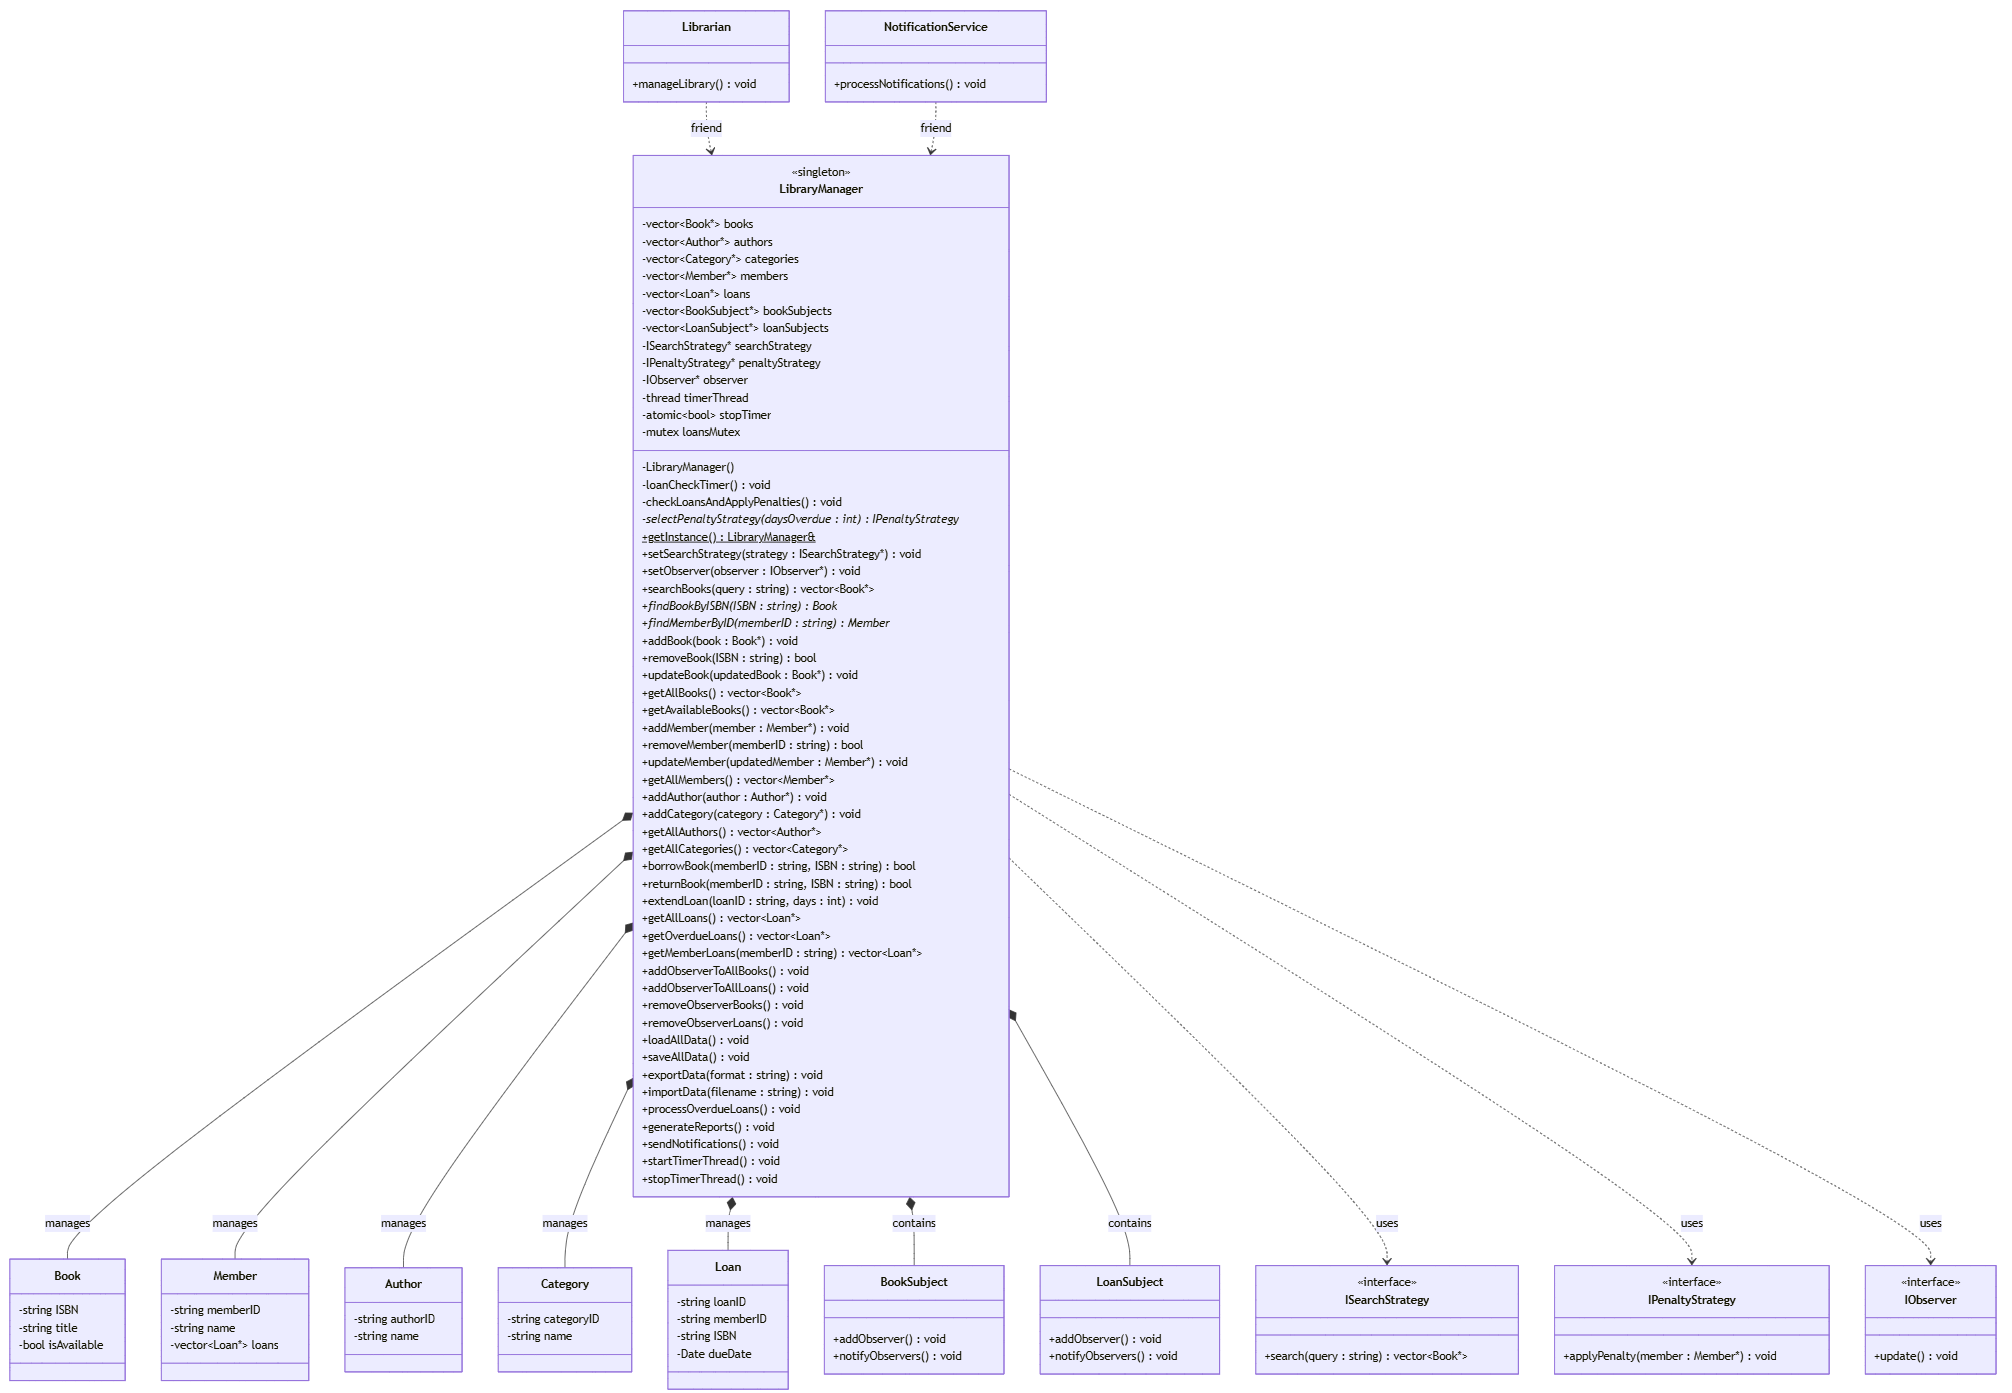
\includegraphics[width=\textwidth]{figures/singleton_pattern.png}
    \caption{UML Diagram showing the combined implementation of Singleton and Facade patterns in LibraryManager.}
    \label{fig:singleton_facade_pattern}
\end{figure}

\newpage

\subsection{Observer Pattern}
\subsubsection{Purpose}
The Observer pattern defines a one-to-many dependency between objects. When one object (the "subject") changes its state, all its dependents (the "observers") are notified and updated automatically. This pattern is ideal for creating distributed event-handling systems.

\subsubsection{Implementation}
The Observer pattern is the backbone of the \texttt{NotificationService}. In our system, entities like \texttt{Loan} act as subjects. Observers, such as a \texttt{MemberObserver} or \texttt{LibrarianObserver}, can register themselves with a subject. When a loan's status changes (e.g., becomes overdue), the loan subject notifies all its registered observers, allowing the system to send alerts or take other actions without tightly coupling the \texttt{Loan} class to the notification logic.

\begin{figure}[H]
    \centering
    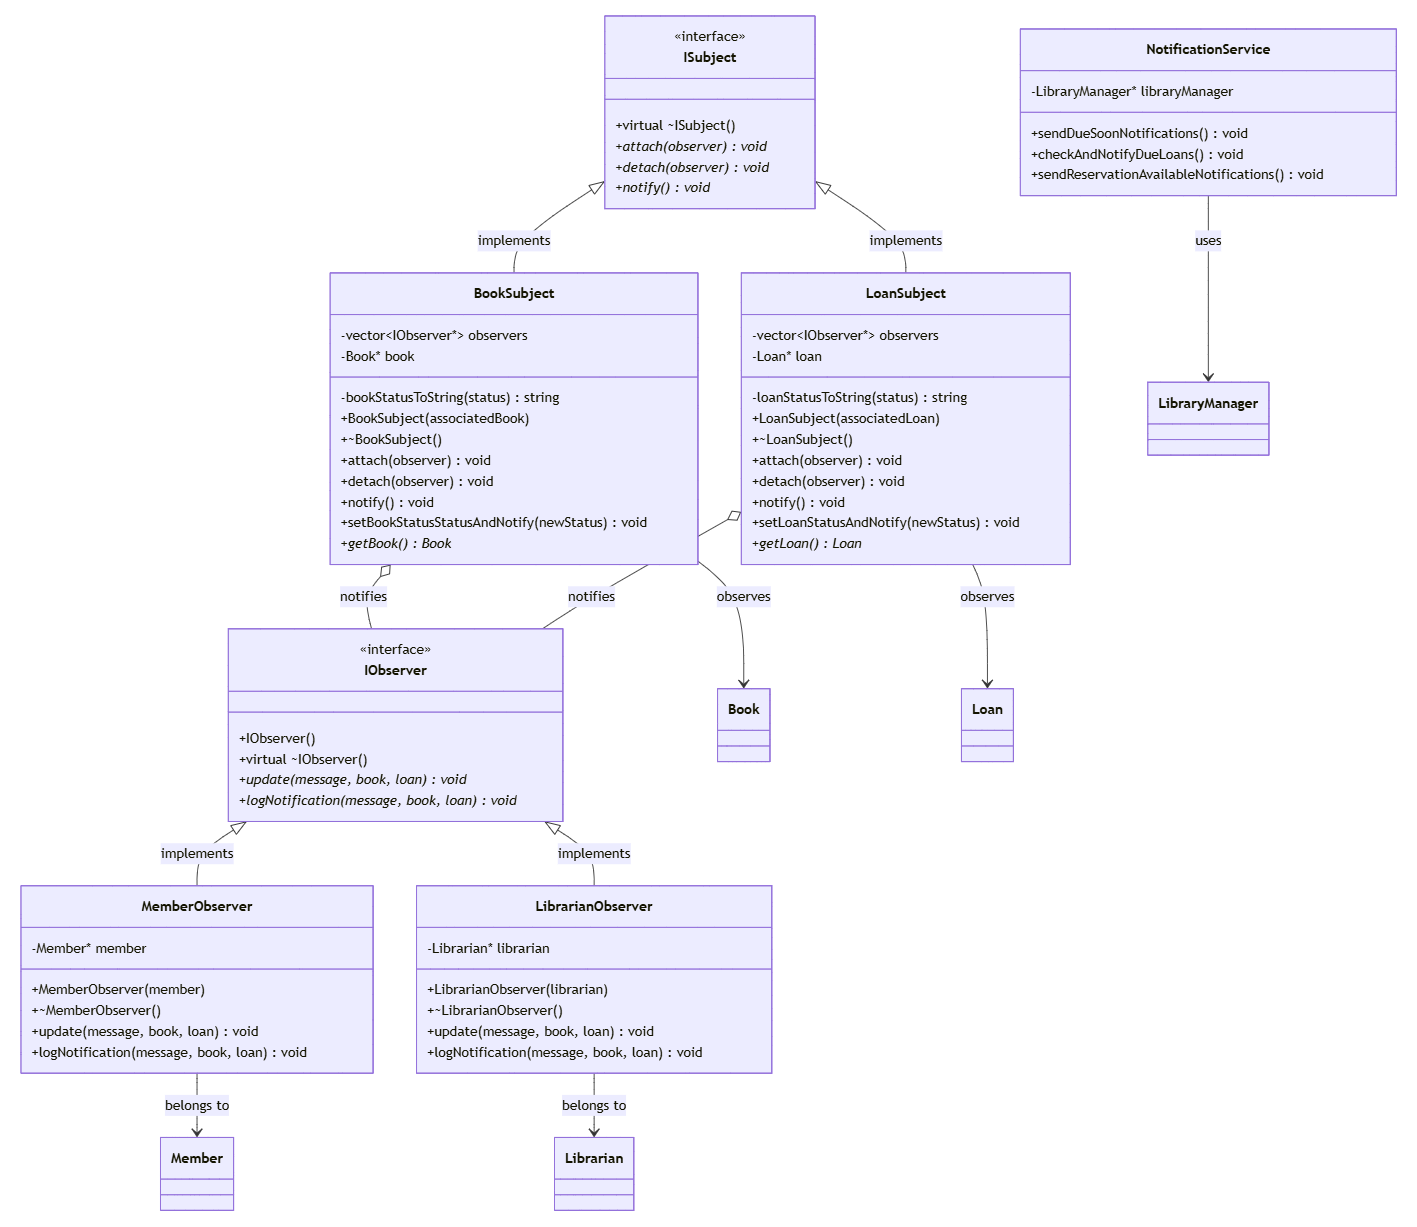
\includegraphics[width=\textwidth]{figures/observer_pattern.png}
    \caption{UML Diagram for the Observer Pattern.}
    \label{fig:observer_pattern}
\end{figure}

\newpage

\subsection{Strategy Pattern}
\subsubsection{Purpose}
The Strategy pattern defines a family of algorithms, encapsulates each one, and makes them interchangeable. It lets the algorithm vary independently from the clients that use it. This is useful when you have multiple ways to perform a task and want to choose one at runtime.

\subsubsection{Implementation}
The Strategy pattern is implemented for two main functionalities: book search operations and penalty calculation systems. 

For search functionality, an abstract interface \texttt{ISearchStrategy} defines a common \texttt{search()} method. Concrete strategy classes like \texttt{TitleSearchStrategy}, \texttt{AuthorSearchStrategy}, and \texttt{ISBNSearchStrategy} implement this interface, each providing a different search algorithm. This allows the system to switch between various search approaches dynamically based on user requirements.

Similarly, for penalty calculations, an abstract interface \texttt{IPenaltyStrategy} defines methods for calculating fines and penalties. Concrete implementations such as \texttt{StandardPenaltyStrategy}, \texttt{StudentPenaltyStrategy}, and \texttt{StaffPenaltyStrategy} provide different penalty calculation algorithms based on member types or library policies. The client code can select and use the desired search or penalty strategy at runtime without being coupled to their specific implementations, promoting flexibility and maintainability.

% --- [HÌNH ẢNH] Sơ đồ cho Strategy Pattern ---
\begin{figure}[H]
    \centering
    % Hãy tạo một ảnh tên là 'strategy_pattern.png' và đặt nó vào thư mục 'figures'
    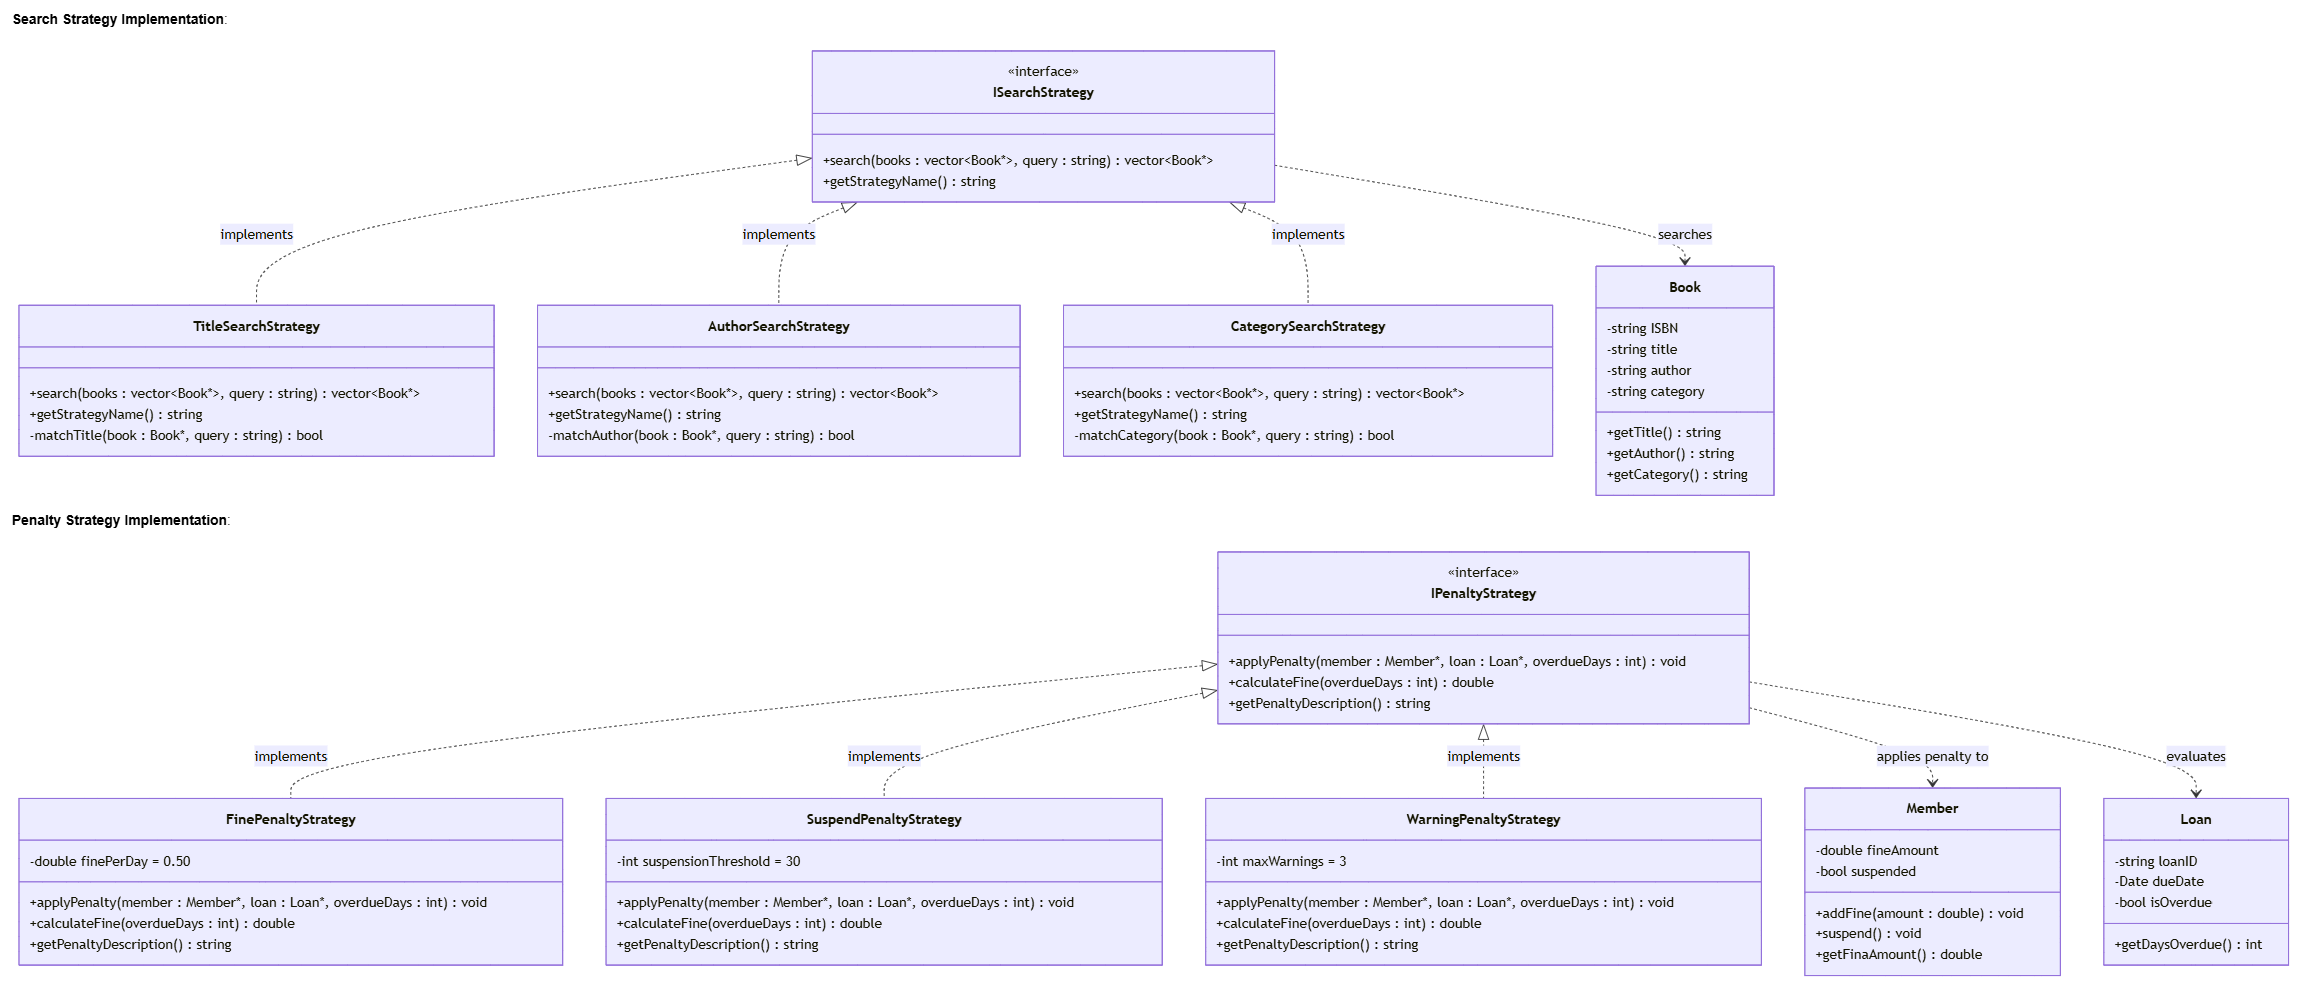
\includegraphics[width=1\textwidth]{figures/strategy_pattern.png}
    \caption{UML Diagram for the Strategy Pattern.}
    \label{fig:strategy_pattern}
\end{figure}

\newpage

\subsection{Decorator Pattern}
\subsubsection{Purpose}
The Decorator pattern allows behavior to be added to an individual object, either statically or dynamically, without affecting the behavior of other objects from the same class. It is used to extend an object's functionality.

\subsubsection{Implementation}
This pattern is used to add extra information to \texttt{Book} objects in a flexible way. A base \texttt{BookDecorator} class inherits from \texttt{Book} and also contains a pointer to a \texttt{Book} object. Concrete decorator classes like \texttt{DifficultyLabelDecorator} and \texttt{SpecialTagDecorator} inherit from \texttt{BookDecorator}. They override methods like \texttt{getFullDescription()} to first call the wrapped object's method and then add their own information (e.g., a difficulty label or a "Bestseller" tag) to the result.

\begin{figure}[H]
    \centering
    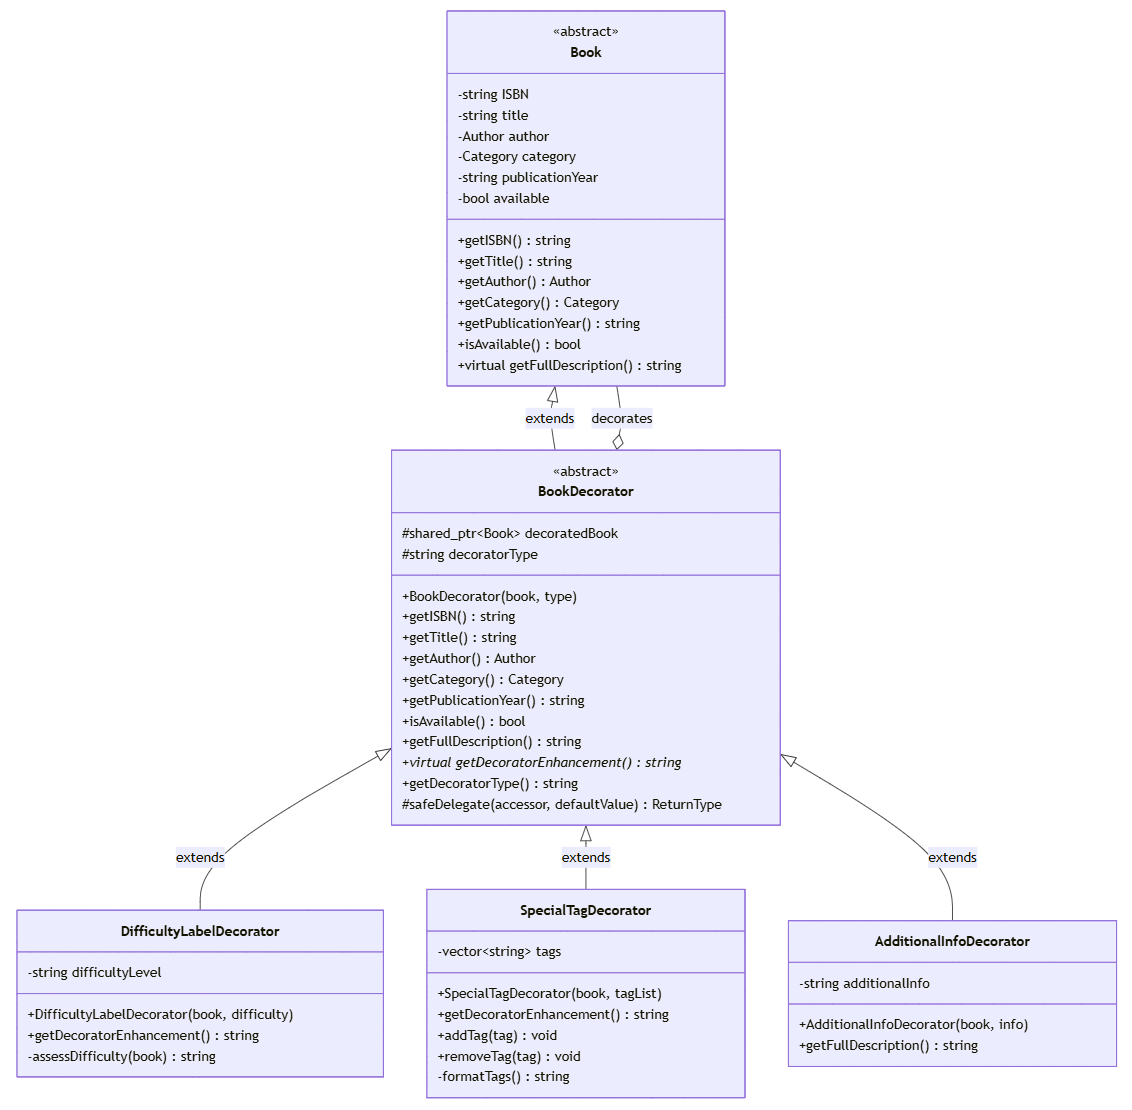
\includegraphics[width=\textwidth]{figures/decorator_pattern.png}
    \caption{UML Diagram for the Decorator Pattern.}
    \label{fig:decorator_pattern}
\end{figure}

\newpage

\subsection{Pattern Integration Benefits}
\subsubsection{Purpose}
The true power of design patterns emerges when they are used in combination rather than isolation. The integration of multiple patterns creates a synergistic effect that enhances the overall system architecture, providing greater flexibility, maintainability, and extensibility than any single pattern could achieve alone.

\subsubsection{Implementation}
The five design patterns work together to create a flexible and robust system:

\begin{itemize}
    \item \textbf{Singleton + Facade:} The \texttt{LibraryManager} serves as both singleton and facade, providing centralized and simplified access to the entire library subsystem while ensuring system-wide consistency.
    
    \item \textbf{Observer + Strategy:} The notification system integrates seamlessly with flexible search and penalty strategies, allowing different algorithms to trigger appropriate notifications based on their specific outcomes.
    
    \item \textbf{Observer + Decorator:} Decorated books can trigger notifications when their enhanced properties change, enabling dynamic response to modifications in book attributes or status.
    
    \item \textbf{Strategy + Decorator:} Different search approaches work effectively with enhanced book information, allowing search strategies to operate on both basic and decorated book properties.
    
    \item \textbf{Facade + Observer:} The simplified interface coordinates complex notification workflows, hiding the complexity of observer management from client code.
    
    \item \textbf{All Patterns Together:} The comprehensive pattern integration creates a clean architecture that promotes maintainability and extensibility, allowing new features to be added with minimal impact on existing code.
\end{itemize}

% This integrated approach demonstrates how design patterns can be combined to address complex software engineering challenges while maintaining code quality and system robustness.

% \begin{figure}[H]
%     \centering
%     \includegraphics[width=\textwidth]{figures/pattern_integration.png}
%     \caption{Overview of pattern integration in the Library Management System.}
%     \label{fig:pattern_integration}
% \end{figure}